%% ------------------------------------------------------------------------- %%
\chapter{Resolução de problemas}
\label{cap:resolucao-problemas}

O intuito deste capítulo é resolver alguns problemas de Maratona de Programação. Resolveremos questões do juíz online SPOJ, um dos mais famosos na Internet, com milhares de problemas disponíveis para praticar. Além de explicar a ideia de como resolver o problema, também apresentaremos pseudocódigos das partes mais cruciais dos problemas. Os códigos completos (em C++) se encontram no GitHub, com a URL específica no fim de cada explicação.

\section{ANTS10 - Colônia de Formigas  (SPOJ Brasil)}

\textit{URL: \url{https://br.spoj.com/problems/ANTS10/}}

\vspace{0.3cm}

\begin{mdframed}[backgroundcolor=blue!5]
\vspace{-0.5cm}

\hspace{0.6cm}{\large{\textbf{Enunciado}}}\vspace{0.2cm}

Um grupo de formigas está muito orgulhoso pois construíram uma grande e magnífica colônia. No entanto, seu enorme tamanho tem se tornado um problema, pois muitas formigas não sabem o caminho entre algumas partes da colônia. Elas precisam de sua ajuda desesperadamente!

A colônia de formigas foi criada como uma série de $N$ formigueiros conectados por túneis. As formigas, obssessivas como são, numeraram os formigueiros sequencialmente à medida que os construiam. O primeiro formigueiro, numerado $0$, não necessitava nenhum túnel, mas para cada um dos formigueiros subsequentes, $1$ até $N-1$, as formigas também construíram um único túnel que conectava o novo formigueiro a um dos formigueiros existentes. Certamente, esse túnel era suficiente para permitir que qualquer formiga visitasse qualquer formigueiro já construído, possivelmente passando através de outros formigueiros pelo percurso, portanto elas não se preocupavam em fazer novos túneis e continuavam construindo mais formigueiros.

O seu trabalho é, dada a estrutura de uma colônia e um conjunto de consultas, calcular, para cada uma das consultas, o menor caminho entre pares de formigueiros. O comprimento do caminho é a soma dos comprimentos de todos os túneis que necessitam ser visitados.

\vspace{0.75cm}{\large{\textbf{Entrada}}}\vspace{0.2cm}

Cada caso de teste se estende por várias linhas. A primeira linha contém um inteiro $N$ representando a quantidade de formigueiros na colônia $(2 \leq N \leq 105)$. Cada uma das próximas $N-1$ linhas contém dois inteiros que descrevem um túnel. A linha $i$, para $1 \leq i \leq N-1$, contém $Ai$ e $Li$, indicando que o formigueiro $i$ foi conectado diretamente ao formigueiro $Ai$ por um túnel de comprimento $Li$ $(0 \leq Ai\leq i-1$ e $1 \leq Li \leq 109)$. A próxima linha contém um inteiro $Q$ representando o número de consultas que seguem $(1 \leq Q \leq 105)$. Cada uma das $Q$ linhas seguintes descreve uma consulta e contém dois inteiros distintos $S$ e $T$ $(0 \leq S,T \leq N-1)$, representando, respectivamente, os formigueiros de origem e destino.

O último caso de teste é seguido por uma linha contendo apenas um zero.

\vspace{0.75cm}{\large{\textbf{Saída}}}\vspace{0.2cm}

Para cada caso de teste, imprima uma única linha com $Q$ inteiros, os comprimentos do menor caminho entre os dois formigueiros de cada consulta. Escreva os resultados para cada consulta na mesma ordem em que aparecem na entrada.

\vspace{0.75cm}

\begin{minipage}{.4\linewidth}
    {\large{\textbf{Exemplo de entrada}}}\vspace{0.2cm}
    \begin{mdframed}[backgroundcolor=gray!10]
        \vspace{-0.5cm}
        6\\
        0 8\\
        1 7\\
        1 9\\
        0 3\\
        4 2\\
        4\\
        2 3\\
        5 2\\
        1 4\\
        0 3\\
        2\\
        0 1\\
        2\\
        1 0\\
        0 1\\
        6 \\
        0 1000000000\\
        1 1000000000\\
        2 1000000000\\
        3 1000000000\\
        4 1000000000\\
        1\\
        5 0\\
        0
        \vspace{-0.4cm}
    \end{mdframed}
\end{minipage}
\hspace{2cm}
\begin{minipage}{.4\linewidth}
    \vspace{-11.25cm}
    {\large{\textbf{Exemplo de saída}}}\vspace{0.2cm}
    \begin{mdframed}[backgroundcolor=gray!10]
        \vspace{-0.5cm}
        16 20 11 17\\
        1 1\\
        5000000000
        \vspace{-0.4cm}
    \end{mdframed}
\end{minipage}%

\vspace{-0.4cm}
\end{mdframed}

\vspace{10cm}

Neste problema, é dado uma árvore com peso nas arestas. Nosso problema consiste em determinar o comprimento do menor caminho entre dois formigueiros $a$ e $b$ - em outras palavras, a soma dos pesos das arestas escolhidas para chegar de $b$ partindo de $a$. Como vimos anteriormente, dado que nosso grafo é uma árvore, só existe um caminho entre quaisquer dois vértices. Portanto, não temos que considerar vários caminhos e ter de fazer algum algoritmo ótimo que escolha o melhor deles - basta percorrer o único caminho e determinar seu comprimento.

Como estudamos, o \LCA\ entre $a$ e $b$ \textbf{sempre} estará contido nos vértices do caminho entre $a$ e $b$. Assim, podemos quebrar o problema de determinar o comprimento total de $a$ até $b$ nos seguintes subproblemas:

\begin{itemize}
    \item Calcular o comprimento do caminho de $a$ até o \LCA(a, b)
    \item Calcular o comprimento do caminho de $b$ até o \LCA(a, b)
\end{itemize}

Vamos então agora analisar a árvore do exemplo da entrada do problema e a primeira consulta feita (comprimento do caminho entre os vértices $2$ e $3$):

\begin{figure}[htb]
\begin{center}
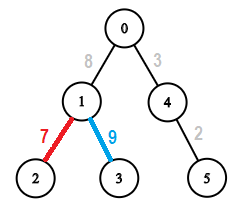
\includegraphics[width=5cm]{images/ants10-graph.png}
\end{center}
\caption{\label{fig:arvore-euler2}Exemplo de entrada do problema com o comprimento do caminho de  $2$ a $3$}
\end{figure}

O \LCA\ entre os vértices $2$ e $3$ é o nó $1$. Assim, o comprimento total do caminho é o tamanho do caminho $(1, 2)$ somado ao tamanho do caminho $(1, 3)$. No caso, $9 + 7 = 16$, que é de fato a resposta para a primeira consulta.

Entretanto, como podemos determinar o tamanho do caminho entre o \LCA\ e todos outros vértices de maneira eficiente? Afinal, poderíamos sempre "descer"\ na árvore a partir do \LCA\ somando os pesos das arestas - ação que custaria $O(n)$ pois no pior caso teríamos que visitar todos os vértices.

A solução para isso é semelhante ao problema de encontrar a soma dos valores em um intervalo consecutivo de números em uma lista. Suponha que temos a seguinte lista:

\begin{center}
    $[4, 10, 5, 6, 8, 2, 1, 3]$
\end{center}

E queremos a soma do intervalo de índices $[3, 6]$ (indexando a lista do 1). Ao invés de iterar a lista inteira somando os números do intervalo (algoritmo $O(n)$), podemos gerar uma lista das somas acumuladas dos números seguindo a seguinte recorrência:

\begin{center}
    $soma[1, i] = soma[1, i-1] + valor[i]$
\end{center}

Assim, o resultado deste algoritmo para a lista apresentada é a nova lista:

\begin{center}
    $[4, 14, 19, 25, 33, 35, 36, 39]$
\end{center}

Ou seja, cada posição agora é a soma de seu valor com todos os outros que o antecede. Para determinar $soma[e, d]$, basta fazer $soma[d] - soma[e-1]$. Assim, estamos somando a lista inteira até a posição mais a direita e subtraindo a soma do começo até o último elemento antes do nosso limite esquerdo da lista, pois essa parte não faz parte do nosso intervalo desejado. Então no caso dos índices $[3, 6]$, temos que:

\begin{center}
    $soma[3, 6] = soma[1, 6] - soma[1, 2] = 35 - 14 = 21$\\
\end{center}

Voltando ao nosso problema, adaptaremos essa técnica para calcular a soma dos pesos das arestas do caminho da raiz até cada vértice da árvore com uma simples DFS:

\begin{algorithm}[H]
\caption{Calculando a soma dos pesos da raiz até todo vértice}
\begin{algorithmic}[1]
\Function{\textsc{CalculaSoma}}{vertice, somaAtual}
    \State $soma[vertice] \rec somaAtual$
    \For{cada $filho$ em $filhos[vertice]$}
        \State $CalculaSoma(filho, somaAtual + comprimento[vertice, filho])$
    \EndFor
\EndFunction
\end{algorithmic}
\end{algorithm}

Basta chamar a função $CalculaSoma$ com a raiz e $0$ (pois o custo de chegar na raiz partindo da raiz é zero). Teremos os seguintes valores de $soma$ (em azul) para cada vértice:

\begin{figure}[htb]
\begin{center}
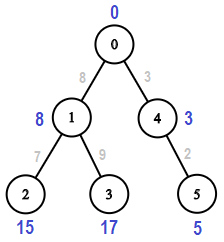
\includegraphics[width=4cm]{images/ants10-graph2.png}
\end{center}
\caption{\label{fig:arvore-euler2}Soma acumulada de cada vértice}
\end{figure}

Agora finalmente conseguimos calcular o comprimento do caminho entre quaisquer dois vértices $a$ e $b$ da seguinte maneira:

\begin{center}
$comprimentoCaminho[a, b] = soma[a] - soma[b]$
\end{center}

Para a consulta do comprimento do caminho $(2, 3)$, temos:
\begin{center}
$caminho(2, 1) = soma[2] - soma[1] = 15 - 8 = 7$\\
$caminho(3, 1) = soma[3] - soma[1] = 17 - 8 = 9$\\
$caminho(2, 3) = caminho (2, 1) + caminho(3, 1) = 7 + 9 = 16$
\end{center}

Pronto! Após o pré-processamento (calcular $soma[i]$ para cada vértice) conseguimos responder cada consulta em $O(log\ n)$ - a complexidade de obter o \LCA\ entre dois vértices, já que o comprimento do caminho é obtido em $O(1)$ (fazer a subtração das somas).

\vspace{0.5cm}

O código completo (em C++) para este problema encontra-se no GitHub:

\url{https://github.com/PedroBortolli/TCC/blob/master/codes/problemas/ANTS10.cpp}

\vspace{10cm}

\section{QTREE2 - Query on a tree II  (SPOJ)}

\textit{URL: \url{https://www.spoj.com/problems/QTREE2/}}

\vspace{0.3cm}OBS: o enunciado original do problema está escrito em inglês. O texto abaixo foi traduzido para a língua portuguesa.\vspace{0.3cm}

\begin{mdframed}[backgroundcolor=blue!5]
\vspace{-0.5cm}

\hspace{0.6cm}{\large{\textbf{Enunciado}}}\vspace{0.2cm}

É dada uma árvore (um grafo conectado acíclico não direcionado) com $N$ vértices, e arestas numeradas $1, 2, 3...N-1$. Cada aresta tem um valor inteiro associado à ela, representando o seu tamanho.

Responda perguntas das seguintes formas:

\begin{itemize}
    \item \textbf{DIST a b}: distância entre os vértices $a$ e $b$
    \item \textbf{KTH a b k}: $k-$ésimo vértice no caminho de $a$ até $b$
\end{itemize}

\vspace{0.35cm}{\large{\textbf{Entrada}}}\vspace{0.2cm}

A primeira linha da entrada contém um inteiro $t$, o número de casos de teste ($t \leq 25$). Então, $t$ casos de testes seguem. Para cada caso de teste: \vspace{0.1cm}

Na primeira linha é dado um inteiro $N$ ($N \leq 10000$)

Nas pŕoximas $N-1$ linhas, a $i-$ésima linha descreve a $i-$ésima aresta: três inteiros $a$ $b$ $c$ denotam uma aresta entre $a$ e $b$ com custo $c$ ($c \leq 100000$).

As próximas linhas contêm perguntas da forma \textbf{"DIST a b"} ou \textbf{"KTH a b k"}

O fim de cada caso de teste é indicado por uma string \textbf{"DONE"}

Existe uma linha em branco entre sucessivos testes

\vspace{0.75cm}{\large{\textbf{Saída}}}\vspace{0.2cm}

Para cada pergunta "DIST" ou "KTH", escreva um inteiro - o resultado da consulta.

Imprima uma linha em branco após cada caso de teste.

\vspace{0.75cm}

\begin{minipage}{.4\linewidth}
    {\large{\textbf{Exemplo de entrada}}}\vspace{0.2cm}
    \begin{mdframed}[backgroundcolor=gray!10]
        \vspace{-0.5cm}
        1\\

        6\\
        1 2 1\\
        2 4 1\\
        2 5 2\\
        1 3 1\\
        3 6 2\\
        DIST 4 6\\
        KTH 4 6 4\\
        DONE
        \vspace{-0.4cm}
    \end{mdframed}
\end{minipage}
\hspace{2cm}
\begin{minipage}{.4\linewidth}
    \vspace{-4.55cm}
    {\large{\textbf{Exemplo de saída}}}\vspace{0.2cm}
    \begin{mdframed}[backgroundcolor=gray!10]
        \vspace{-0.5cm}
        5\\
        3
        \vspace{-0.4cm}
    \end{mdframed}
\end{minipage}%

\vspace{-0.4cm}
\end{mdframed}

Neste problema queremos duas coisas:

\begin{itemize}
    \item Distância entre dois vértices $a$ e $b$
    \item Descobrir o $k-$ésimo vértice no caminho de $a$ até $b$
\end{itemize}

A primeira consulta já foi analisada no problema anterior desta seção, então não discutiremos sobre ela novamente aqui. O foco agora é descobrir como responder o segundo tipo de consulta de forma ótima - isto é - melhor do que o jeito trivial $O(n)$ de percorrer o caminho inteiro vértice a vértice.

Como estudamos no capítulo 5, sabemos que conseguimos chegar em qualquer vértice $v$ a partir de um nó fazendo sucessivos pulos de "tamanho potência de dois". Em outras palavras, qualquer número pode ser representado como uma soma de potências de dois diferentes.

Portanto, a sugestão para resolver este problema é utilizar o método de programação dinâmica para obter a resposta: pré-calcular os ancestrais 1, 2, 4, 8, etc níveis acima de todo vértice da árvore.

Assim, para obter o $k-$ésimo vértice temos que considerar dois casos:

\begin{itemize}
    \item Ele pode estar contido no caminho de $a$ até o \LCA($a, b$). Isso acontece se $profundidade[a] - profundidade[\LCA] + 1 \geq k$. Ou seja, se a quantidade de vértices neste caminho é maior ou igual a $k$, então o $k-$ésimo nó está contido neste caminho
    \item Senão, ele está contido no caminho de $b$ até o \LCA($a, b$)
\end{itemize}

Agora, sabendo em qual caminho devemos procurar, podemos utilizar os ancestrais de potência de dois já pré-calculados para obter nossa resposta. Vamos supor que o $k-$ésimo vértice está no caminho de $a$ até o \LCA. Podemos, a partir do nó $a$, executar o algoritmo de subir sucessivas potências de dois até alcançar o vértice que está $k-1$ níveis acima de si (pois quando $k = 1$ o vértice a ser retornado é o próprio $a$). Por exemplo, quando $k = 4$, sabemos que queremos o vértice $3$ níveis acima de $a$. Assim, podemos obter o vértice $2$ níveis acima de $a$, e depois o vértice $1$ nível acima deste novo nó encontrado. O resultado será o vértice $2 + 1 = 3$ níveis acima de $a$.

\begin{figure}[htb]
\begin{center}
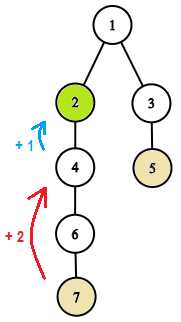
\includegraphics[width=4.25cm]{images/qtree2-graph.png}
\end{center}
\caption{\label{fig:arvore-euler2}Obtenção do quarto vértice no caminho de 7 até 5}
\end{figure}

Seja $quantidadeA$ o número de vértices no caminho de $a$ até o \LCA($a, b$) e $quantidadeB$ o número de vértices do caminho de $b$. No caso em que o $k-$ésimo vértice encontra-se no caminho de $b$ até o \LCA($a, b$), o que queremos agora é o vértice que está $k - quantidadeA$ níveis \textbf{abaixo} do \LCA. Entretanto, nosso pré-processamento apenas computa os ancestrais de um vértice - em outras palavras - os nós que se encontram acima de um vértice. Assim, precisamos transformar o nosso problema em encontrar um vértice \textbf{acima} de $b$, e podemos fazer isso da seguinte forma:

\begin{center}
$alvo = quantidadeA + quantidadeB - k$    
\end{center}

Agora o valor da variável $alvo$ é a quantidade de níveis que precisamos subir a partir de $b$ para encontrar o $k-$ésimo vértice do caminho de $a$ até $b$.

\begin{algorithm}[H]
\caption{Encontrando o $k-$ésimo vértice do caminho de $a$ até $b$}
\begin{algorithmic}[1]
\Function{\textsc{KVertice}}{a, b}
    \State $lca \rec LCA(a, b)$
    \State $quantidadeA \rec profundidade[a] - profundidade[lca] + 1$
    \State $quantidadeB \rec profundidade[b] - profundidade[lca]$
    \If {$k \leq quantidadeA$}
        \State $alvo \rec k - 1$
        \State $i \rec logNiveis$
        \While { $i \geq 0$}
            \If {$2^i \leq alvo$}
                \State $alvo \rec alvo - 2^i$
                \State $a = pd[a][i]$
            \EndIf
        \EndWhile
        \Return $a$
    \Else
        \State $alvo \rec quantidadeA + quantidadeB - k$
        \State $i \rec logNiveis$
        \While { $i \geq 0$}
            \If {$2^i \leq alvo$}
                \State $alvo \rec alvo - 2^i$
                \State $b = pd[b][i]$
            \EndIf
        \EndWhile
        \Return $b$
    \EndIf
\EndFunction
\end{algorithmic}
\end{algorithm}

Desta forma, conseguimos encontrar o $k-$ésimo vértice de um caminho em $O(log\ n)$.

\vspace{0.5cm}

O código completo (em c++) para este problema encontra-se no GitHub:

\url{https://github.com/PedroBortolli/TCC/blob/master/codes/problemas/QTREE2.cpp}

\vspace{0.3cm}
